% ===== This file generates all figures for the JCIIOT 2026 Competition Paper =====
% Run this with: pdflatex create_figures.tex
% Output: individual PNG/PDF files in figures directory

\documentclass[tikz,border=10pt]{standalone}
\usepackage{tikz}
\usetikzlibrary{shapes,arrows.meta,positioning,calc,backgrounds,shadows.blur}

% ===== Define Styles =====
\tikzstyle{block} = [rectangle, draw, fill=blue!10, text width=8em, text centered, rounded corners, minimum height=3em, blur shadow]
\tikzstyle{line} = [draw, -Stealth, thick]
\tikzstyle{cloud} = [draw, ellipse, fill=red!20, minimum height=2.5em, blur shadow]
\tikzstyle{process} = [rectangle, draw, fill=orange!10, text width=10em, text centered, minimum height=2.5em, blur shadow]
\tikzstyle{dataflow} = [->, thick, >={Stealth[length=4pt]}]

% ===== Main Figure: System Architecture Diagram =====
\begin{document}

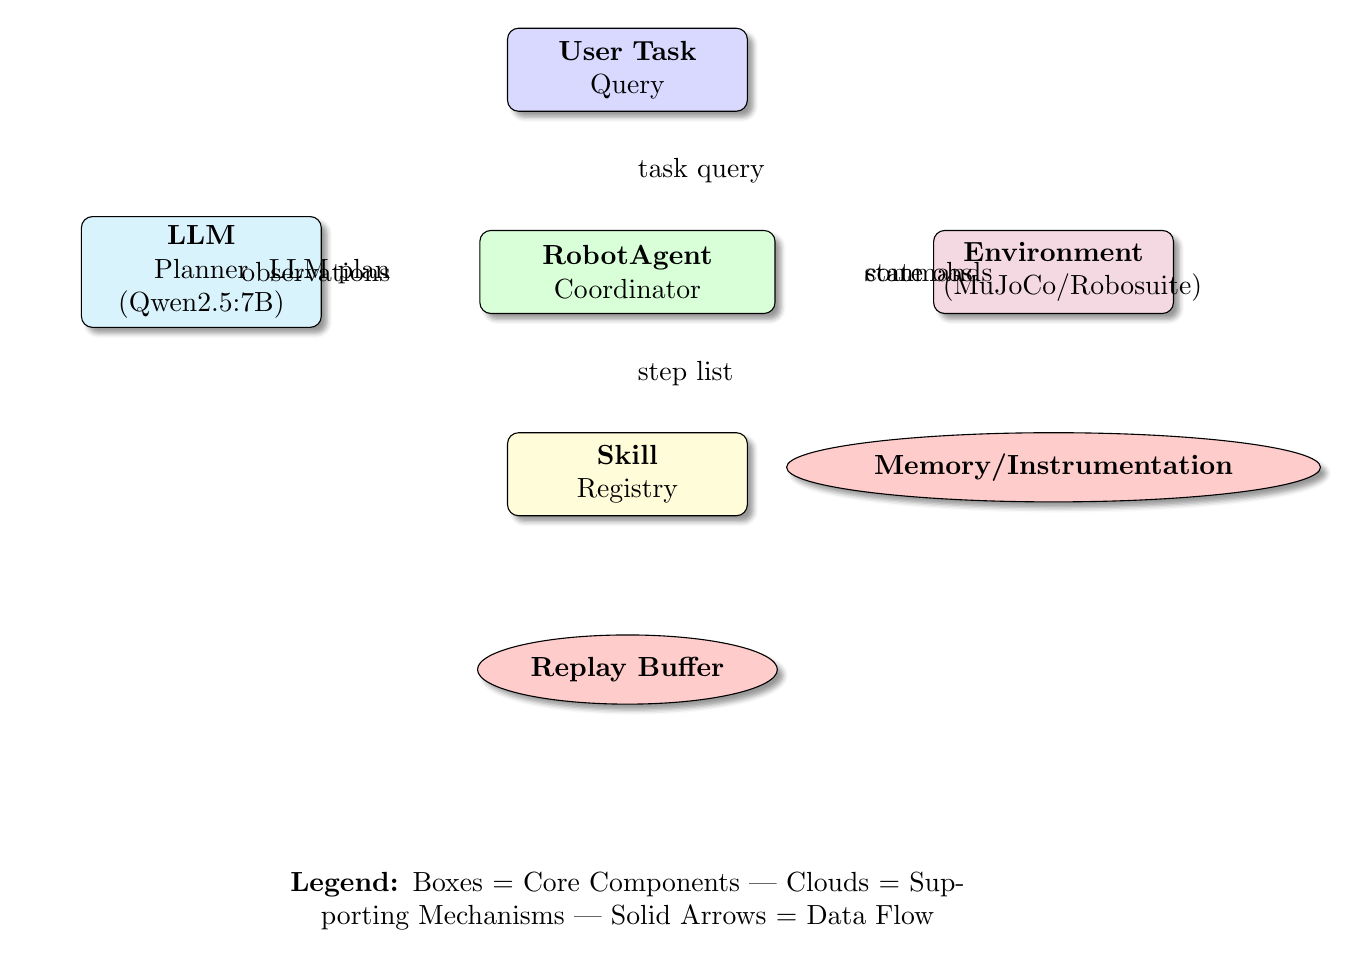
\begin{tikzpicture}[node distance=1.5cm and 2cm, auto, >=Stealth]

% Central RobotAgent block
\node[block, text width=10em, fill=green!15] (robotagent) {\textbf{RobotAgent}\\ Coordinator};

% Top: User Input
\node[block, above=of robotagent, fill=blue!15] (userinput) {\textbf{User Task}\\ Query};

% Bottom: Skills Registry
\node[block, below=of robotagent, fill=yellow!15] (skillsreg) {\textbf{Skill}\\ Registry};

% Left: Planner
\node[block, left=of robotagent, fill=cyan!15] (planner) {\textbf{LLM}\\ Planner\\(Qwen2.5:7B)};

% Right: Environment
\node[block, right=of robotagent, fill=purple!15] (environment) {\textbf{Environment}\\(MuJoCo/Robosuite)};

% Below environment: Memory
\node[cloud, below=of environment] (memory) {\textbf{Memory/Instrumentation}};

% Below skillsreg: Replay
\node[cloud, below=of skillsreg] (replay) {\textbf{Replay Buffer}};

% Arrows
\path[dataflow] (userinput) -- node{task query} (robotagent);
\path[dataflow] (robotagent) -- node{step list} (skillsreg);
\path[dataflow] (robotagent) -- node[left]{observations} (planner);
\path[dataflow] (planner) -- node[left]{LLM plan} (robotagent);
\path[dataflow] (robotagent) -- node[right]{commands} (environment);
\path[dataflow] (environment) -- node[right]{state obs} (robotagent);
\path[dataflow] (robotagent) -- node{} (memory);
\path[dataflow] (skillsreg) -- node{} (replay);

% Legend
\node[text width=15cm, text centered, below=2cm of replay] {
\textbf{Legend:} Boxes = Core Components | Clouds = Supporting Mechanisms | Solid Arrows = Data Flow
};

\end{tikzpicture}

\end{document}
